\documentclass[tikz,border=8pt]{standalone}
% Shared look for every TikZ diagram. Load with \input{../../tools/tikz-style.tex}
\usepackage[sfdefault]{roboto}
\usetikzlibrary{arrows.meta, positioning, shapes.geometric, calc, fit, backgrounds}
\definecolor{cblue}{HTML}{4C78A8}
\definecolor{corange}{HTML}{F58518}
\definecolor{cgreen}{HTML}{54A24B}
\definecolor{cred}{HTML}{E45756}
\definecolor{cpurple}{HTML}{B279A2}
\definecolor{cgrey}{HTML}{6B6B6B}
\tikzset{
  every picture/.style={font=\sffamily, line width=1.2pt},
  box/.style={draw=#1, fill=#1!12, rounded corners=4pt, align=center, inner sep=7pt, minimum height=1.1cm},
  box/.default=cgrey,
  arrow/.style={-{Stealth[length=3mm]}, draw=cgrey, line width=1.4pt},
  title/.style={font=\sffamily\bfseries\Large},
  note/.style={font=\sffamily\small, text=cgrey, align=center},
}
\AtBeginDocument{\hyphenpenalty=10000 \exhyphenpenalty=10000}

% Why the look-ahead point sees the heading: the car's rear axle is 0.5 m left of the course (offset e = 0.5 m) and
% heads 0.1 rad (5.7 deg) to the left of it (heading error). 4 m along its heading it would be 0.5 + 4 x 0.1 = 0.9 m
% left of the course, so the look-ahead point on the course lies about 0.9 m to the right of the heading line
% (exactly 0.894 m, notebook). Sideways distances are drawn twice as large as forward ones.
\begin{document}
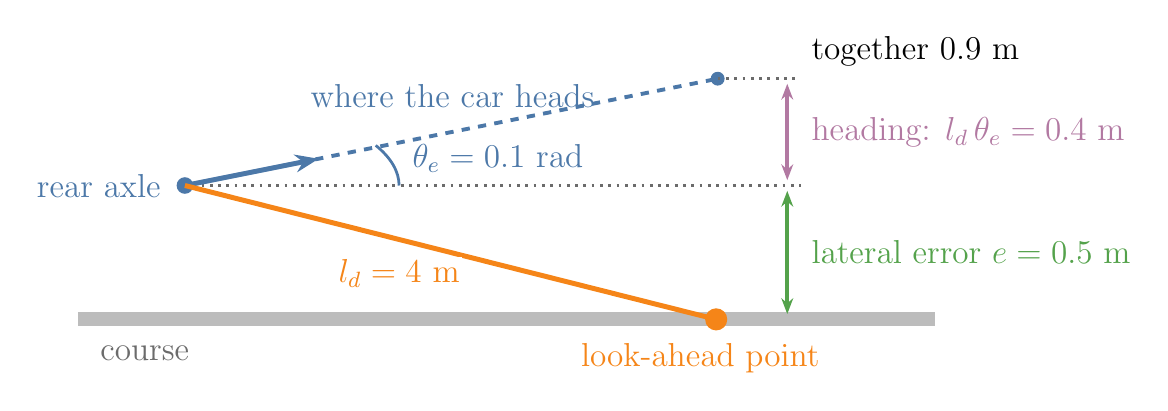
\begin{tikzpicture}[x=1.7cm, y=3.4cm, every node/.append style={font=\large}]
  % course
  \draw[cgrey!45, line width=5pt] (-0.8,0) -- (5.6,0);
  \node[cgrey, anchor=north] at (-0.3,-0.06) {course};
  % the car's rear axle and a line parallel to the course through it
  \draw[cgrey, dotted, line width=1pt] (0,0.5) -- (4.6,0.5);
  \fill[cblue] (0,0.5) circle[radius=3pt];
  \node[cblue, anchor=east] at (-0.1,0.5) {rear axle};
  % heading line, 4 m long
  \draw[cblue, dashed, line width=1.4pt] (0,0.5) -- (3.98,0.899);
  \draw[-{Stealth[length=3mm]}, cblue, line width=1.8pt] (0,0.5) -- (1.0,0.6);
  \node[cblue, anchor=south] at (2.0,0.75) {where the car heads};
  \fill[cblue] (3.98,0.899) circle[radius=2.5pt];
  % heading error angle
  \draw[cblue, line width=1pt] (1.6,0.5) arc[start angle=0, end angle=27, x radius=1.6, y radius=0.33];
  \node[cblue, anchor=west] at (1.62,0.6) {$\theta_e = 0.1$ rad};
  % chord to the look-ahead point
  \draw[corange, line width=1.8pt] (0,0.5) -- (3.969,0);
  \fill[corange] (3.969,0) circle[radius=4pt];
  \node[corange, anchor=north] at (3.85,-0.05) {look-ahead point};
  \node[corange, anchor=north, fill=white, inner sep=1pt] at (1.6,0.24) {$l_d = 4$ m};
  % the split of the sideways gap
  \draw[cgreen, line width=1.6pt, {Stealth[length=2mm]}-{Stealth[length=2mm]}] (4.5,0.02) -- (4.5,0.48);
  \draw[cpurple, line width=1.6pt, {Stealth[length=2mm]}-{Stealth[length=2mm]}] (4.5,0.52) -- (4.5,0.88);
  \draw[cgrey, dotted, line width=1pt] (3.98,0.899) -- (4.6,0.899);
  \node[cgreen, anchor=west, align=left] at (4.6,0.25) {lateral error $e = 0.5$ m};
  \node[cpurple, anchor=west, align=left] at (4.6,0.7) {heading: $l_d\thinspace\theta_e = 0.4$ m};
  \node[black, anchor=west, align=left] at (4.6,1.0) {together 0.9 m};
\end{tikzpicture}
\end{document}
